
\section{Electromagnetic Induction with Sinusoidal Fields}

\makelabheader %(Space for student name, etc., defined in master.tex)

\bigskip

\textbf{Introduction}

In this lab, we'll take a further look at Faraday's Law, which says
that a changing magnetic field can produce an emf (that is, a voltage)
in a loop of wire.  Current will be supplied to a large coil (which is a 
series of loops of wire), resulting in a magnetic field.  
If the current were constant in time,
then a steady magnetic field would be produced.  Since we want to
produce a changing magnetic field, we supply the coil with {\it
alternating current}, that is, current that flows back and forth in
alternating directions, oscillating in a sinusoidal (sine-wave) fashion.  The
result is an ever-changing magnetic field, which induces an emf in
a separate small coil.

\begin{wrapfigure}[16]{r}{0.5\textwidth}
\vspace{0.4in}

\hspace{0.4in}
    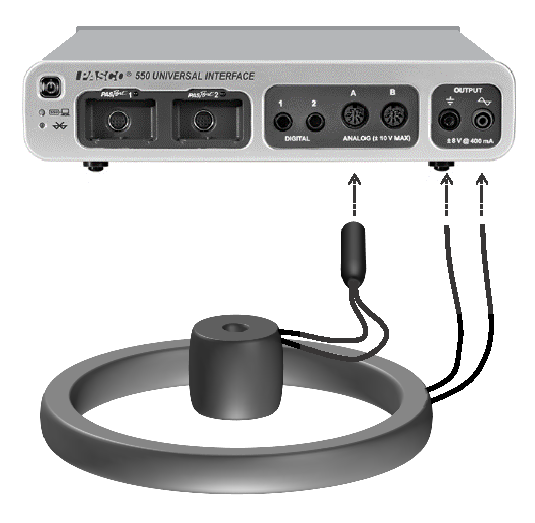
\includegraphics[width=0.4\textwidth]{induction_sinusoidal/induction2_setup_550.eps}
\end{wrapfigure}

\bigskip

\textbf{Apparatus}
\begin{itemize}
\setlength\itemsep{0pt} %Spacing on this page is awkward; setting these lengths manually at least looks ok.  --MT
\item one large wire coil
\item one small wire coil
\item two banana plug leads with alligator clips
\item Pasco 550 interface
\item voltage probe
\item \textit{Capstone} software (\filename{Induction2.cap} experiment file)
\end{itemize}

\medskip
\textbf{Setup}

Connect the large coil to the output
terminals on the right side of the interface using banana plug wires and 
alligator clips). These output terminals supply alternating current to the 
large coil. Connect the small coil to the ``voltage 
sensor'' (really just an over-priced adapter), and plug it into port A on the interface. Place the small coil in 
the center of the large coil as shown.
\bigskip

\textbf{Activity 1: Qualitative Predictions} 

The top graph on the 
following page shows the current flowing through the large 
coil as a function of time. When $I$ is positive, that means current is 
flowing in one direction around the coil, and when $I$ is negative the current 
is flowing in the other direction. 

On the axes below the top graph, use dotted lines to sketch your predictions of the 
shapes of the following other quantities.
(Don't worry about the overall scale on the vertical axis;
just focus on the shapes of the graphs, and particularly the locations
of the peaks and valleys.  Hint: some of the graphs will be exactly
the same shape as the given graph of $I$.)

\begin{enumerate}
\item
On the first set of axes, sketch the vertical component of the magnetic field,
$B_z$, at the center of the large coil (realizing that this field is directly
proportional to the current in the coil).
\item On the the next set of axes, sketch the magnetic flux $\Phi_ B$ passing
through the small coil. (This flux is proportional to the magnetic field 
produced in the large coil).
\item On the bottom set of axes, sketch the emf ${\cal E}$ induced in the small
coil (which, by Faraday's law, is proportional to the negative time derivative 
of the flux through the coil).
\end{enumerate}

%\begin{center}
%    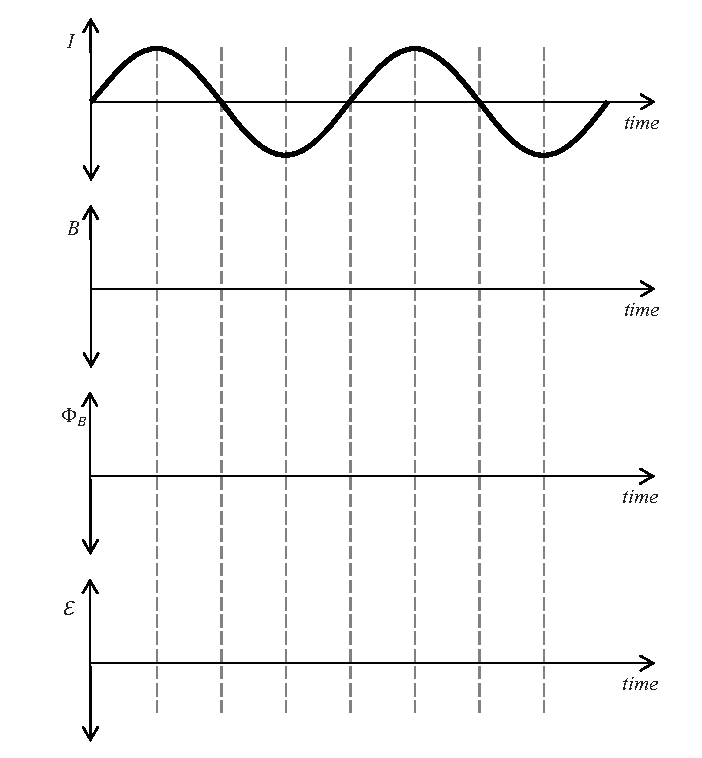
\includegraphics[width=0.7\textwidth]{induction_sinusoidal/sine_curve.eps}
%\end{center}

\begin{lab_groupplot}*{\makegroupverticals[4]{90,180,270,360,450,540,630,720}{0}{770}}
					[lab_noticks_2quads,
	height=1.2in,width=4in,
	xmin=0,xmax = 770,
 	group style={
		group size=1 by 4,
		vertical sep=0.2in
		},
	xlabel=time $t$,
	]
\nextgroupplot[ylabel={Current $I(t)$}]
	\addplot +[domain=0:720] {0.85*sin(x) }; %Why is it calculating sine in degrees?
\nextgroupplot[ylabel={Magnetic Field $B(t)$}]
\nextgroupplot[ylabel={Flux $\Phi(t)$}]
\nextgroupplot[ylabel={emf $\varepsilon(t)$}]
\end{lab_groupplot}

The computer will measure and graph
the current $I(t)$ in the large coil, and the emf ${\cal E}(t)$
in the small coil.  We want to test whether the two graphs are related
to each other in the way you predicted.  To be specific, make the following
predictions from your graphs before trying the experiment:

\begin{enumerate}[labparts]
\item At times when $I(t)$ is at its maximum value, what is ${\cal E}$?
\answerspace{.7in}

\item At times when $I(t)$ is at its minimum value, what is ${\cal E}$?
\answerspace{.7in}

\item At times when $I(t)=0$, what is ${\cal E}$?
\answerspace{.7in}
\end{enumerate}

\pagebreak[2]

{\bf Activity 2: Testing the Predictions}

Open the file \filename{Induction2.cap} in the \filename{\coursefolder} folder.  You should see two graphs,
one showing the current in the large coil and one showing the emf (voltage)
across the small coil.  Both graphs will be blank until you start taking
data, of course.  
%There should be an additional box that allows you to control the frequency of oscillation of the alternating current.  Leave this alone for now; we'll mess around with it later.

Hit the Record button and take data for about 5 seconds.  

\begin{enumerate}[labparts]
\item Do the shapes of the
two graphs generally match your predictions from Activity 1? (To answer this, you may want to expand the scales of the horizontal axes of the graphs so you can see the shapes better.  Be sure to align the graphs so that the times are synchronized.) 

\answerspace{1in}

\textit{If the answer to this question is ``yes,'' then go on.  If it's ``no,
the shape of the second one is exactly the opposite of what I expected,''
then you just have the small coil upside-down; turn it over and 
try again.  If the answer is not one of those two, then consult your 
instructor.}

\item  Sketch the actual shape of ${\cal E}(t)$ using a solid line on the last graph on the previous page.
\medskip

\item  Let's be a bit more specific in comparing the predictions
with the data.  Examine the current graph, and record the
times of the first two or three moments when the current reaches a maximum.
Then look at the other graph, and record the emf at those same two or three times.
Are the results consistent with your prediction in part (a) of Activity 1?

\answerspace{0.9in}

\item  Perform a similar analysis to check your predictions in (b) and (c) of Activity 1.
In each case, check several appropriately-chosen moments of time to see
if the relationship between $I$ and ${\cal E}$ is as you predicted.

\answerspace{1in}

\item  Suppose that you rotate the small coil 90$^\circ$, so that its axis
is horizontal.  What do you predict about the resulting emf ?
\answerspace{0.8in}

\item  Test your prediction and record the results here.  Did your result match your prediction?
\answerspace{0.8in}
\end{enumerate}

\pagebreak[2]

\textbf{Activity 3: A More Quantitative Analysis}

In the previous activities, we just looked at the shapes of the graphs, without worrying
about the exact details.  In this activity we'll do things a bit more precisely.

\begin{enumerate}[labparts]
\item Suppose we have a wire, carrying current $I$, that is bent into a circular loop of radius $R$.  What will be the magnitude of the magnetic field $B_z$ at the center of the circle? (Answer in terms of $I$ and $R$ and any other physical constants like $\mu_0$.)
\answerspace{1.2in}

\item The big coil you have been using is basically a big circle of wire, carrying a current given by the equation
$$
I(t)=I_{\rm max}\sin(2\pi f t).
$$
Here $I_{\rm max}$ is the maximum value of the current, and
$f$ is the frequency (that is, the number of cycles per second).  
Your big coil also has multiple turns of wire to make the magnetic field bigger.
Assuming that your coil consists of $N_1$ circular loops of
wire, each with radius $R$, write down a similar expression for
the magnetic field $B_z(t)$ at the center of the coil.
\answerspace{0.8in}

\item Now suppose that the small coil has area $A$.  Write down an expression for $\Phi_B(t)$, the
flux through the small coil.
\answerspace{0.75in}

\item Assuming the small coil consists of $N_2$ loops of wire, use Faraday's law to write an expression 
for ${\cal E}(t)$, the emf induced in the small coil.
\answerspace{0.75in}

\item What is the maximum emf ${\cal E}_{\rm max}$?  Express your prediction
in terms of quantities such as $I_{\rm max},f,A,N_1,N_2,R$.
\answerspace{0.75in}

\item Rearrange this expression so that it has the quantities ${\cal E}_{\rm max}$,
$I_{\rm max}$, and $f$ on the left-hand side, and everything else on the right.
\answerspace{0.75in}


\pagebreak[3]
We will now try an experiment in which we vary the frequency $f$.  We'll
find that this results in changes in both the current and the emf.
But note that everything on the right-hand side of the above expression
must remain constant throughout this experiment.  That
means that the expression on the left must also remain
constant.  We will test this prediction.

\item  To find the frequency of the generator, click on the icon on the left labeled ``Signal Generator.''  Record the frequency $f$ from that panel, and also the maximum current $I_{\rm max}$ and the
maximum emf ${\cal E}_{\rm max}$ from the data on your two graphs.
Then, use the ``Signal Generator'' panel to change the frequency to a higher value,
and record these three quantities again.  Repeat this a total of four
times, so that you have four sets of values $f, I_{\rm max}, {\cal E}_{\rm max}$.
Take care not to move the coils from one run to the next.
\answerspace{3in}

\item  You made a prediction above that a certain combination of these
three quantities would remain constant throughout this experiment.
Calculate that quantity for each of the four data runs.  Are the
results consistent with your prediction?
\answerspace{3in}
\end{enumerate}

